As we said in the first section, the product taken into analysis is a seasonal item. Using Google Trends, we were able to identify the region of maximum and minimum interest of the users regarding a Louis Vuitton scarf. In the graph below is clear that this product is searched primarily in the cold seasons and it is year after year more demanded by the customers. In the chart the x-axis represents a five year time period while the y-axis represents the popularity of the keywords "Louis Vuitton Scarf" searched on Google (100 is the moment of maximum interest while 0 is the minimum).
\makebox[\textwidth][c]{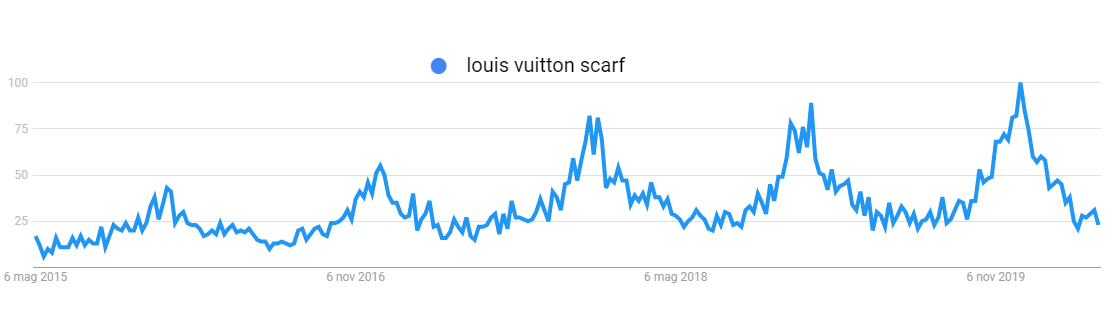
\includegraphics[width=1.2\textwidth]{sections/images/trend}}
Based on the diagram we decided to divide the year in four periods of time, each one underlining a different phase.\newline\\
\makebox[\textwidth][c]{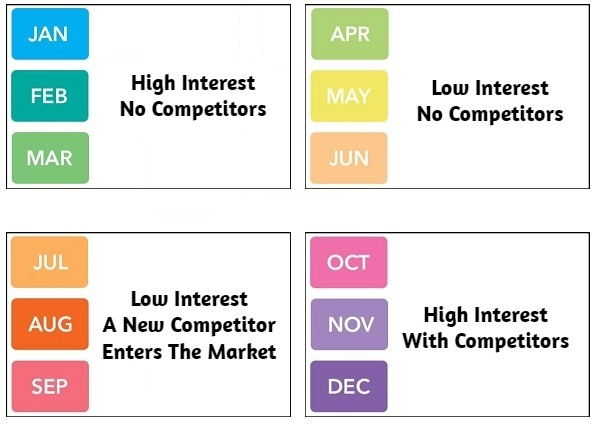
\includegraphics[width=0.8\textwidth]{sections/images/months}}
In order to better understand our reasoning behind the decisions that brought us to choose as graphs for the four different phases the ones showed below, is important to notice some remarks. \\In the first phase (Jan-Feb-Mar) the growth of the curve is almost linear, since there are no competitors that can interfere with our advertising of the product. However, there is a large pool of users to influence, since it is a phase of high interest of the product.\\\\
\makebox[\textwidth][c]{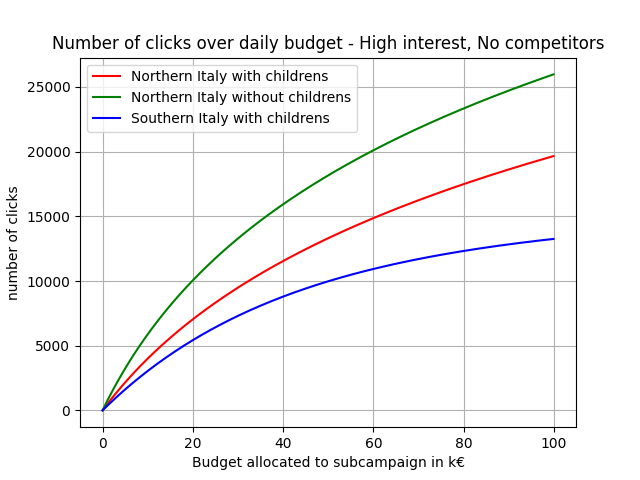
\includegraphics[width=0.85\textwidth]{../curves/real_curves/daily_clicks_10}} \newpage
In the second phase (Apr-May-Jun) instead, since in these months the interest about the item is low, there will be less people interested in the scarf, therefore the impact that a higher budget allocated to the ads can make is less relevant than the impact that it can produce on a high interest phase. Based on this assumption we decided that the graph for the second phase should have a more remarkable growth with a small budget allocated to the ads, settling to much more slower growth as the budget significantly increases. \\\\
\makebox[\textwidth][c]{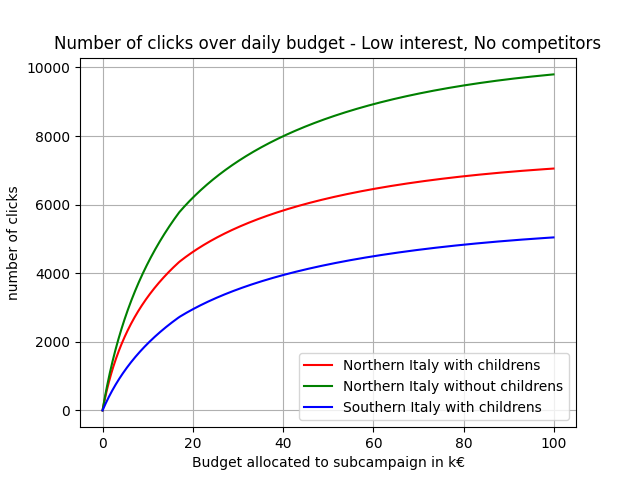
\includegraphics[width=0.85\textwidth]{../curves/real_curves/daily_clicks_00}} \newpage
In the next phase (Jul-Aug-Sep), when the new competitor enters the market, the graph is different in the low budget allocated range with respect to the second graph, while maintaining a similar profile in the high budget allocated range. The cause is the following: since we need to beat the competition in order to sell our product, we would struggle to do so allocating a small amount of money to the advertisement, while instead allocating a sufficient amount of money to a certain class, we should be able to attract more user of this class. \\\\
\makebox[\textwidth][c]{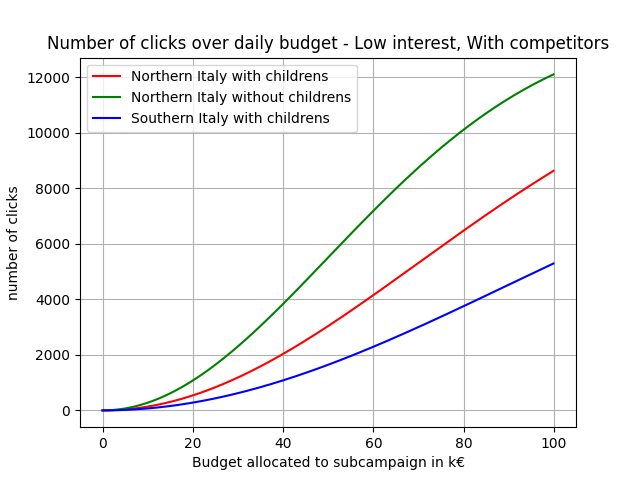
\includegraphics[width=0.85\textwidth]{../curves/real_curves/daily_clicks_01}} \newpage
Finally, in the last phase (Oct-Nov-Dec) we focused on the fact that since it is an high interest phase, this time with a competitor that challenges us, the budget that needs to be allocated to each sub-campaigns still needs to be a considerable amount if we want to attract a sufficient number of users as in the third phase. However, in this period the pool of users that can be reached is much wider, translating into a more linear curve in the high budget allocated range with respect to the third phase.\\\\
\makebox[\textwidth][c]{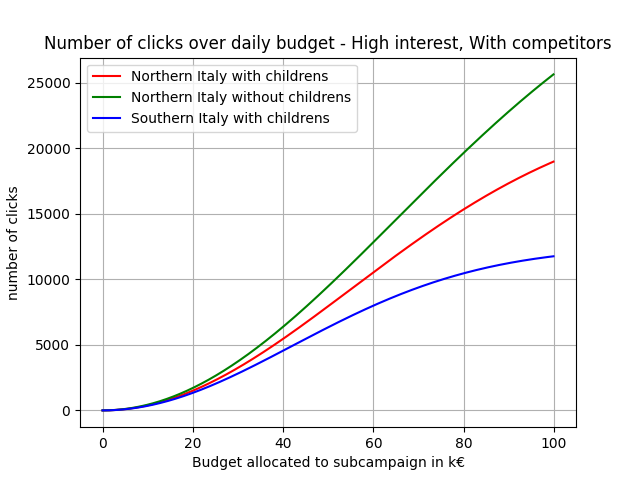
\includegraphics[width=0.85\textwidth]{../curves/real_curves/daily_clicks_11}} \\\\
